% See exam.cls and examdoc.tex for the license information
\documentclass[12pt, answers]{exam}

\usepackage{amssymb}
\usepackage{makeidx}
\usepackage{amsmath}
\usepackage{graphicx}
\usepackage{caption}
\usepackage{tabulary}
\usepackage{color}
\usepackage{multicol}
\usepackage{multirow}
\usepackage{enumerate}
\usepackage{float}
\usepackage{colortbl}
\usepackage[table,xcdraw]{xcolor}
\usepackage{array}

\newcolumntype{C}[1]{>{\centering\let\newline\\\arraybackslash\hspace{0pt}}m{#1}}

\addpoints

% In case we're not using hyperref.sty:
\providecommand{\texorpdfstring}[2]{#1}
% The following can be used in \section commands
% without generating pdf warnings:
\newcommand{\bs}{\texorpdfstring{\char`\\}{}}

\makeindex

\newcommand{\indc}[1]{\index{#1@\texttt{\char`\\#1}}}
\newcommand{\indcsub}[2]{\index{#1@\texttt{\char`\\#1}!#2}}
\newcommand{\indcstart}[1]{\index{#1@\texttt{\char`\\#1}|(}}
\newcommand{\indcstop}[1]{\index{#1@\texttt{\char`\\#1}|)}}

\newcommand{\indt}[1]{\index{#1@\texttt{#1}}}
\newcommand{\indtsub}[2]{\index{#1@\texttt{#1}!#2}}
\newcommand{\indtstart}[1]{\index{#1@\texttt{#1}|(}}
\newcommand{\indtstop}[1]{\index{#1@\texttt{#1}|)}}

\extraheadheight{-.4in}

\pagestyle{headandfoot}
%\extraheadheight{.2 in}
\firstpageheader{}{}{}
\runningheader{}{}{}
\firstpagefooter{}{Model evaluation}{Page \thepage\ of \numpages}
\firstpagefootrule
\runningfooter{}{Model evaluation}{Page \thepage\ of \numpages}
\runningfootrule

%---------------------------------------------------------------------

\shadedsolutions
\noprintanswers
\definecolor{SolutionColor}{rgb}{0.8,0.9,1}

\setcounter{section}{4}

\begin{document}

\section{Exercises -- Model evaluation}

%---------------------------------------------------------------------
\begin{questions}

%%% Question 1
\question \textbf{Basic measures from confusion matrix}
  
The oval representation below shows that a model has classified a test data set with 10 positives and 10 negatives and produced four outcomes.
 
\begin{figure}[H]
      \centering
      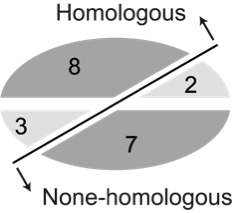
\includegraphics[width=0.2 \textwidth]{fig07/oval_representation.png}
\end{figure}

\vspace{0.1 in}

\begin{parts}

%% (a)
  \part Fill each blank cell with one of the four classification outcomes - TP, FP, TN, and FN.

\begin{table}[H]
\centering
\begin{tabular}{ll|c|c|}
\cline{3-4}
                                                            &                & \multicolumn{2}{c|}{Test data}                                        \\ \cline{3-4} 
                                                            &                & \multicolumn{1}{l|}{Homologous} & \multicolumn{1}{l|}{Non-homologous} \\ \hline
\multicolumn{1}{|l|}{\multirow{2}{*}{Model classification}} & Homologous     &                                 &                                     \\ \cline{2-4} 
\multicolumn{1}{|l|}{}                                      & Non-homologous &                                 &                                     \\ \hline
\end{tabular}
\end{table}

%% (b)
\part Make a confusion matrix from the oval representation above.

\begin{table}[H]
\centering
\begin{tabular}{ll|c|c|}
\cline{3-4}
                                                            &                & \multicolumn{2}{c|}{Test data}                                        \\ \cline{3-4} 
                                                            &                & \multicolumn{1}{l|}{Homologous} & \multicolumn{1}{l|}{Non-homologous} \\ \hline
\multicolumn{1}{|l|}{\multirow{2}{*}{Model classification}} & Homologous     &                                 &                                     \\ \cline{2-4} 
\multicolumn{1}{|l|}{}                                      & Non-homologous &                                 &                                     \\ \hline
\end{tabular}
\end{table}

%% (c)
  \part Calculate the following basic evaluation measures for the oval representation. Round off the answer to two decimal places if necessary.
  
\bigskip 
Accuracy
$= \dfrac{TP+TN}{P+N} $

\bigskip 
Error rate
$= \dfrac{FP+FN}{P+N} $

\bigskip 
Sensitivity
$= \dfrac{TP}{P} $

\bigskip 
Specificity
$= \dfrac{TN}{N} $

\bigskip 
Precision
$=\dfrac{TP}{TP+FP}$


\end{parts}



%%% Question 2
\question \textbf{Measures with multiple thresholds}
  
Create multiple confusion matrices by considering all possible threshold values. Assume that the test data set contains two positives and two negatives. The table below shows the scores given by a model that gives higher scores for the alignments with higher similarities. 

\begin{table}[H]
\centering
\begin{tabular}{|l|l|l|l|l|}
\hline
Test set label & P   & P   & N   & N   \\ \hline
Model score    & 2.1 & 3.1 & 2.3 & 1.2 \\ \hline
\end{tabular}
\end{table}

\vspace{0.1 in}

\begin{parts}

%% (a)
  \part Fill the labels that match the sorted scores

\begin{figure}[H]
      \centering
      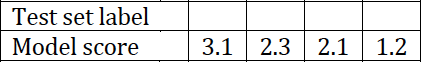
\includegraphics[width=0.4 \textwidth]{fig07/sorted_test.png}
\end{figure}

%% (b)
\part Fill the labels predicted by different threshold values.

\begin{figure}[H]
      \centering
      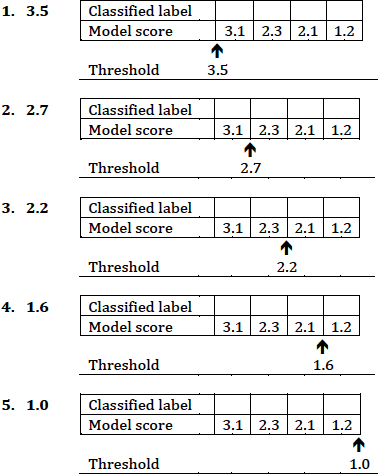
\includegraphics[width=0.6 \textwidth]{fig07/thresholds.png}
\end{figure}

%
% NEWPAGE
%
\newpage

%% (c)
  \part Use the labels in (a) and (b) and calculate TP, FP, TN, and FN for all threshold values.

\begin{table}[H]
\centering
\begin{tabular}{|l|l|l|l|l|}
\hline
Threshold & TP & FP & TN & FN \\ \hline
3.5       &    &    &    &    \\ \hline
2.7       &    &    &    &    \\ \hline
2.2       &    &    &    &    \\ \hline
1.6       &    &    &    &    \\ \hline
1         &    &    &    &    \\ \hline
\end{tabular}
\end{table}

%% (d)
  \part Use the result in (c) and calculate basic evaluation measures. Round off the answer to one decimal place if necessary.

\begin{table}[H]
\centering
\begin{tabular}{|l|l|l|l|}
\hline
Threshold & Specificity & 1 - specificity & Sensitivity \\ \hline
3.5       &             &                 &             \\ \hline
2.7       &             &                 &             \\ \hline
2.2       &             &                 &             \\ \hline
1.6       &             &                 &             \\ \hline
1         &             &                 &             \\ \hline
\end{tabular}
\end{table}

%% (e)
  \part Draw a ROC curve for the calculated evaluation measures in (d).

\begin{figure}[H]
      \centering
      
\includegraphics[width=0.3 \textwidth]{fig07/roc.png}
\end{figure}

%% (f)
  \part Calculate the area under the curve of the curve in (e).
  
\begin{solution}[0.35 in]
0.75
\end{solution}

%% (g)
  \part Evaluate the ROC curve in your own words.
  
\begin{solution}[0.35 in]
The model performs better than random classifiers
\end{solution}

\end{parts}



\end{questions}
%---------------------------------------------------------------------
       
\end{document}

